%Minimierung leer Thread
\subsection{Minimierung von Threads im Leerlauf }

In CUDA  arbeiten gleichzeitig 32 Threads auf einem Multiprozessor.
%gleichzeitig mit 32 Threads \cite{cudapg}.
Diese gehören alle zum selben Block.
Bei der Sparsematrix-Multiplikation sind viele Threads im Leerlauf.
Um die Anzahl der leerlaufenden Threads zu minimieren,
müssen mehrere Punktprodukte in einem Block bearbeitet werden.
Dazu verwendet man zweidimensionale Blocksizes.
Die Definition und Anwendung zweidimensionaler Blocksizes findet man in \cite{cudapg} und \cite{cudbp}.

% \begin{figure}[htbp]
	% 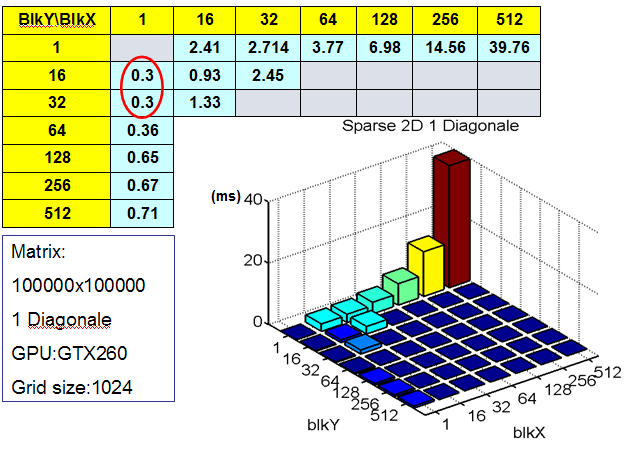
\includegraphics[width=1.7in]{../xby/pic//einDiagonal}
	% \caption{Multipliktion Ein-Diagonalematrize mal Vektor. BlockY: Anzahl der Y-Dimension von Block; BlockX: Anzahl der X-Dimension von Block}
	% 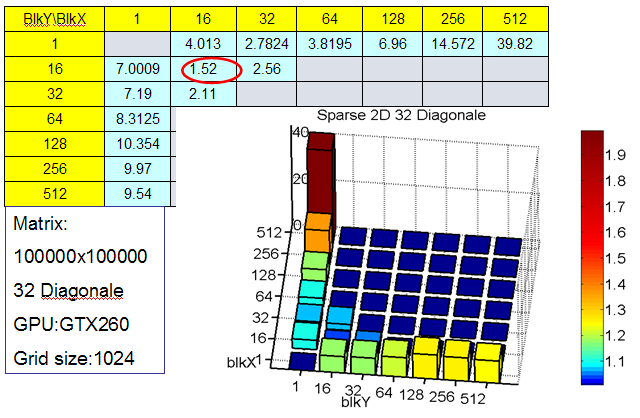
\includegraphics[width=1.7in]{../xby/pic//moreDiagonal}
	% \caption{Multipliktion 32-Diagonalematrize mal Vektor. BlockY: Anzahl der Y-Dimension von Block; BlockX: Anzahl der X-Dimension von Block.}
% \end{figure}